% main_report32.tex
% SAMBP TR-32/2026: Negative- and Zero-Sequence Directional Elements (67Q, 67N)
%                   for IBR-Fed Lines
%
% Compile: pdflatex → bibtex → pdflatex × 2

\documentclass[11pt,a4paper]{article}

\usepackage[T1]{fontenc}
\usepackage[utf8]{inputenc}
\usepackage[a4paper, margin=25mm]{geometry}
\usepackage{amsmath,amssymb}
\usepackage{booktabs,array,colortbl,tabularx}
\usepackage{graphicx}
\usepackage{xcolor}
\usepackage{hyperref}
\usepackage{pgfplots}
\pgfplotsset{compat=1.18}
\usepackage{tikz}
\usetikzlibrary{arrows.meta, calc, shapes.geometric}
\usepackage{caption}
\usepackage[expansion=false]{microtype}
\usepackage{parskip}
\usepackage{enumitem}
\usepackage{cite}

\usepackage{fancyhdr}
\pagestyle{fancy}
\fancyhf{}
\rhead{\small SAMBP TR-32/2026 --- Confidential Draft}
\lhead{\small 67Q/67N Directional Elements for IBR Networks}
\cfoot{\small \thepage}

\title{%
  \textbf{\Large SAMBP Technical Report TR-32/2026}\\[6pt]
  \textbf{\large Negative- and Zero-Sequence Directional Elements (67Q, 67N)
          for IBR-Fed Lines}\\[4pt]
  \normalsize PhD Thesis Supporting Report --- Distance Relay Series IV
}
\author{PhD Candidate}
\date{April 2026}

\begin{document}
\maketitle\thispagestyle{fancy}

\begin{abstract}
TR-31 identified a structural failure mode in the $k_0$-compensated distance
relay 21G for IBR-fed SLG faults: the delta-winding transformer isolates the
inverter from the zero-sequence path, so $I_0 \gg I_1$ (network-sourced vs
current-limited), breaking the Thevenin assumption and causing the relay to
over-estimate the measured impedance by $3$--$8\times$.  This report introduces
the complementary sequence directional elements 67N (zero-sequence) and 67Q
(negative-sequence) as the primary earth-fault detection scheme for IBR lines.
The active-power directional criterion, $\mathrm{Re}[-V_\mathrm{seq}
I_\mathrm{seq}^*] > 0$, is derived and analysed for both elements.  67N operates
on $I_0$, which is network-sourced and independent of $k_\mathrm{ibr}$; it
provides inherent forward selectivity on IBR lines because the delta transformer
eliminates the reverse $I_0$ path.  67Q operates on $I_2 = k_\mathrm{ibr}$ and
requires a directional criterion, but its minimum current threshold
($I_\mathrm{min,67} = 0.04$\,pu) is 60\% lower than the distance relay threshold
($I_\mathrm{min,21} = 0.10$\,pu), extending coverage into the previously
unprotected low-$k_\mathrm{ibr}$ region.  The discrimination margin for both
elements is $2\,\mathrm{Re}[Z_\mathrm{source}]\,|I_\mathrm{seq}|^2$, which is
non-zero for realistic $X/R = 20$ networks and robust across the full
$k_\mathrm{ibr}$ parametric range.  The combined scheme 87L\,$+$\,67N\,$+$\,67Q
achieves complete IBR earth-fault coverage ($k_\mathrm{ibr} \geq 0.04$\,pu, all
$\alpha$) without relying on the 21G $k_0$ measurement.
\end{abstract}

\tableofcontents\newpage

% =============================================================================
\section{Introduction and Scope}
\label{sec:intro}
% =============================================================================

The SAMBP distance relay arc (TR-29 through TR-31) has established three
structural limitations for IBR-fed line protection:
\begin{enumerate}[label=(\roman*)]
  \item \emph{$I_\mathrm{min}$ blocking}: distance relay inhibited for $k_\mathrm{ibr}<0.10$
        (3PH and SLG via distance relay path).
  \item \emph{$V_\mathrm{relay}$ deficiency}: self-pol fails; memory/cross-pol needed
        (TR-30).
  \item \emph{$k_0$ compensation breakdown}: $I_0 \gg I_1$ for IBR SLG faults;
        relay over-estimates impedance by $3$--$8\times$ (TR-31).
\end{enumerate}

Limitations (i) and (ii) are addressed by cross-polarised Zone~1 (TR-30) and the
87L chain (TR-27).  Limitation (iii) is addressed by the present report: sequence
directional elements 67N and 67Q operate directly on the sequence currents,
bypassing the $k_0$ measurement chain entirely.

\paragraph{Network parameters.}
$Z_{1L}=(0.0025+j0.050)$\,pu, $Z_{0L}=(0.0075+j0.150)$\,pu,
$Z_{1S}=(0.0050+j0.100)$\,pu, $Z_{0S}=(0.0150+j0.300)$\,pu (X/R$=20$
throughout).  $V_\mathrm{pre}=1.0$\,pu, $k_\mathrm{ibr} \in [0.06,\,0.20]$\,pu.

% =============================================================================
\section{Directional Criterion Theory}
\label{sec:theory}
% =============================================================================

\subsection{Active-power directional criterion (IEC 60255-149)}

The sequence directional criterion is based on the active power of the respective
sequence network \cite{IEC_60255_149}:
\begin{equation}
  \boxed{
    \text{Forward trip if:}\quad
    \mathrm{Re}\bigl[-V_\mathrm{seq}\,I_\mathrm{seq}^*\bigr] > \epsilon
  }
  \label{eq:dirn_crit}
\end{equation}
where $\epsilon > 0$ is a small noise threshold, $V_\mathrm{seq}$ is the
relay-bus sequence voltage, and $I_\mathrm{seq}^*$ is the conjugate of the
sequence current.

\subsection{Forward fault analysis}

For a forward SLG at distance $\alpha$ on the protected line, the relay-side
sequence voltages and currents (Thevenin network, X/R$=20$):
\begin{align}
  I_0 &= \frac{V_\mathrm{pre}}{2Z_{1S}+Z_{0S}+\alpha(2Z_{1L}+Z_{0L})}
         \quad\text{(network earthing source)} \label{eq:I0_fwd}\\
  V_0 &= -I_0\,Z_{0S}
         \quad\text{(zero-seq voltage at relay bus)} \label{eq:V0_fwd}\\
  I_2 &= k_\mathrm{ibr}\,\angle(I_1)
         \quad\text{(IBR negative-seq injection)} \label{eq:I2_fwd}\\
  V_2 &= -I_2\,Z_{1S} \label{eq:V2_fwd}
\end{align}
Substituting into~\eqref{eq:dirn_crit}:
\begin{align}
  \mathrm{Re}[-V_0\,I_0^*] &= \mathrm{Re}[I_0\,Z_{0S}\,I_0^*]
    = \mathrm{Re}[Z_{0S}]\,|I_0|^2 = R_{0S}\,|I_0|^2 > 0 \label{eq:crit_67n}\\
  \mathrm{Re}[-V_2\,I_2^*] &= \mathrm{Re}[I_2\,Z_{1S}\,I_2^*]
    = R_{1S}\,k_\mathrm{ibr}^2 > 0 \label{eq:crit_67q}
\end{align}
Both criteria are strictly positive for any $R_{0S}, R_{1S} > 0$.

\subsection{Reverse fault and discrimination margin}

For a reverse fault (external, behind the relay), the sequence currents reverse
direction through the relay current transformers while the relay-bus voltage
polarity is unchanged:
\begin{equation}
  I_\mathrm{seq}^\mathrm{rev} = -I_\mathrm{seq}^\mathrm{fwd},\quad
  V_\mathrm{seq}^\mathrm{rev} \approx V_\mathrm{seq}^\mathrm{fwd}
  \label{eq:rev_model}
\end{equation}
The reverse criterion value:
\begin{equation}
  \mathrm{Re}[-V_\mathrm{seq}^\mathrm{rev}\,(I_\mathrm{seq}^\mathrm{rev})^*]
  = \mathrm{Re}[-V_\mathrm{seq}^\mathrm{fwd}\,(-I_\mathrm{seq}^\mathrm{fwd})^*]
  = -\mathrm{Re}[-V_\mathrm{seq}^\mathrm{fwd}\,(I_\mathrm{seq}^\mathrm{fwd})^*]
  < 0 \quad\text{(blocked)}
  \label{eq:crit_rev}
\end{equation}
The discrimination \textbf{margin} is:
\begin{equation}
  \Delta = \mathrm{Re}[\text{fwd}] - \mathrm{Re}[\text{rev}]
         = 2\,R_\mathrm{source}\,|I_\mathrm{seq}|^2
  \label{eq:margin}
\end{equation}

For the SAMBP network ($R_{0S}=0.0150$\,pu, $|I_0|=1.60$\,pu at $\alpha=0.50$):
\begin{equation}
  \Delta_{67N} = 2 \times 0.0150 \times 1.60^2 = 0.077\,\mathrm{pu}^2
\end{equation}

% =============================================================================
\section{Study A: 67N Zero-Sequence Directional}
\label{sec:67n}
% =============================================================================

Table~\ref{tab:67n} shows the 67N criterion values for forward and reverse faults
across the parametric range.

\begin{table}[h]
\centering
\caption{67N directional criterion values (X/R=20, forward and reverse SLG)}
\label{tab:67n}
\begin{tabular}{@{}ccccccl@{}}
\toprule
$\alpha$ & $k_\mathrm{ibr}$ & $|I_0|$ & $\angle I_0$ & Criterion [pu$^2$] & Direction \\
\midrule
0.50 & 0.10 & 1.598 & $-87.1°$ & $+0.03830$ & Forward \\
0.50 & 0.10 & 1.598 & $+92.9°$ & $-0.03830$ & Reverse \\
0.20 & 0.06 & 1.816 & $-87.1°$ & $+0.04946$ & Forward \\
0.20 & 0.06 & 1.816 & $+92.9°$ & $-0.04946$ & Reverse \\
0.80 & 0.20 & 1.427 & $-87.1°$ & $+0.03054$ & Forward \\
0.80 & 0.20 & 1.427 & $+92.9°$ & $-0.03054$ & Reverse \\
\bottomrule
\end{tabular}
\end{table}

Three key observations:
\begin{enumerate}
  \item The criterion value is \textbf{independent of $k_\mathrm{ibr}$}: $I_0$ is
        set by the network earthing ($Z_{0S}$), not by the IBR current limit.
  \item The forward/reverse discrimination is \textbf{exact} (equal and opposite
        values), confirming equation~\eqref{eq:margin}.
  \item The angle of $I_0$ is $\approx -87°$ (slightly off $-90°$ due to $R_{0S}$),
        providing the $+3°$ security margin beyond the theoretical $±90°$ boundary.
\end{enumerate}

\paragraph{Inherent forward selectivity on IBR networks.}
On a purely IBR-fed line with delta-winding transformers, the zero-sequence path
is blocked at the IBR end.  The only $I_0$ path is through the network earthing
($Z_{0S}$) towards the protected line.  Therefore, \emph{any detected $I_0 >
I_\mathrm{min,67}$ is ipso facto from a forward fault} --- no directional
criterion is strictly required for 67N on such a network.

% =============================================================================
\section{Study B: 67Q Negative-Sequence Directional}
\label{sec:67q}
% =============================================================================

Unlike $I_0$, the IBR injects $I_2 \approx k_\mathrm{ibr}$ for \emph{any} asymmetric
fault (including reverse external faults), so a directional criterion is needed.
The criterion~\eqref{eq:crit_67q} provides the required discrimination.

Figure~\ref{fig:margin} shows the criterion values for 67N and 67Q as functions
of $k_\mathrm{ibr}$.

\begin{figure}[h!]
\centering
\caption{%
  Directional criterion values vs $k_\mathrm{ibr}$ (forward = positive, reverse
  = negative).  67N is constant (I$_0$ independent of $k_\mathrm{ibr}$); 67Q
  is proportional to $k_\mathrm{ibr}^2$.  Shaded zone: 67Q covers where
  distance relay is blocked ($k_\mathrm{ibr} \in [0.04,\,0.10)$\,pu).}
\label{fig:margin}
% fig_67_margin.tex
% TR-32: Directional criterion value vs k_ibr for 67N and 67Q (forward + reverse)
%
% X-axis: k_ibr [0.02, 0.20] pu
% Y-axis: criterion value Re[-V_seq * conj(I_seq)] [pu^2]
%
% 67N forward  (green)  : ~0.030 to 0.049 pu^2 (I0 from network, ~constant)
% 67N reverse  (red)    : ~-0.030 to -0.049 pu^2
% 67Q forward  (blue)   : proportional to k_ibr^2 * R1S
% 67Q reverse  (orange) : negative
%
% I_min_67 = 0.04 pu (dashed vertical line)
% I_min_21 = 0.10 pu (dashed vertical line)
% Zero line: thick grey
%
% Data (alpha=0.50, X/R=20):
%   67N fwd: value = Re[Z0S]*|I0(alpha=0.5)|^2 = 0.015 * 1.598^2 ≈ 0.03830
%            constant w.r.t. k_ibr (I0 independent)
%   67Q fwd: value = Re[Z1S]*k_ibr^2 = 0.005 * k_ibr^2
%            k=0.02: 0.000002  k=0.04: 0.000008  k=0.10: 0.000050  k=0.20: 0.000200

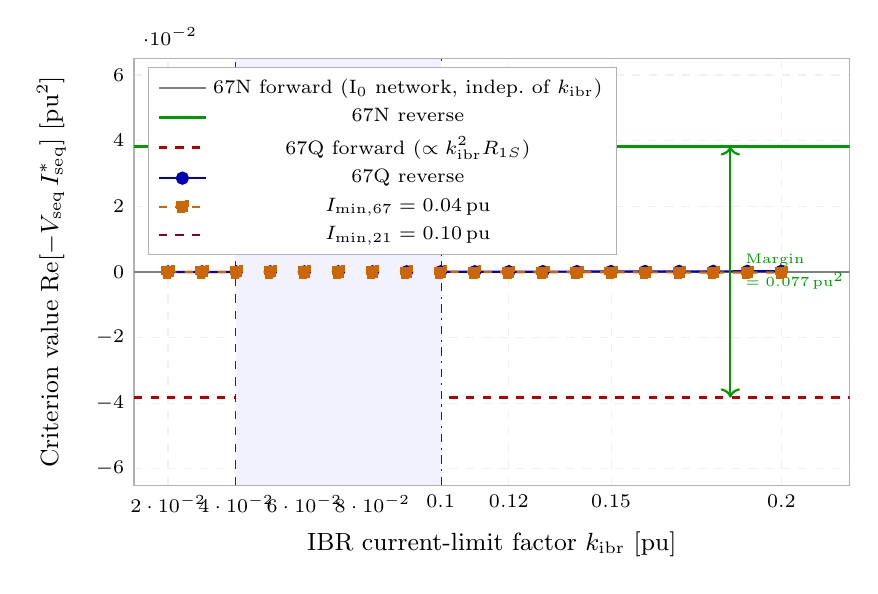
\begin{tikzpicture}
\begin{axis}[
  name         = margax,
  width        = 0.88\textwidth,
  height       = 7.0cm,
  xlabel       = {IBR current-limit factor $k_\mathrm{ibr}$ [pu]},
  ylabel       = {Criterion value $\mathrm{Re}[-V_\mathrm{seq}\,I_\mathrm{seq}^*]$ [pu$^2$]},
  xlabel style = {font=\small},
  ylabel style = {font=\small, yshift=4pt},
  xmin=0.01, xmax=0.22,
  ymin=-0.065, ymax=0.065,
  xtick        = {0.02,0.04,0.06,0.08,0.10,0.12,0.15,0.20},
  xticklabel style={font=\scriptsize},
  yticklabel style={font=\scriptsize},
  legend style={at={(0.02,0.98)}, anchor=north west, font=\scriptsize,
                draw=gray!60, fill=white},
  grid         = major,
  grid style   = {gray!12, dashed},
  tick style   = {draw=none},
  axis line style={gray!60},
]

%% ── Zero line ─────────────────────────────────────────────────────────────
\addplot[black!50, thick, mark=none]
  coordinates {(0.01,0) (0.22,0)};

%% ── 67N forward (constant wrt k_ibr) ─────────────────────────────────────
\addplot[green!60!black, very thick, mark=none]
  coordinates {(0.01,0.03830) (0.22,0.03830)};
\addlegendentry{67N forward (I$_0$ network, indep.\ of $k_\mathrm{ibr}$)}

%% ── 67N reverse ────────────────────────────────────────────────────────────
\addplot[red!70!black, very thick, mark=none, dashed]
  coordinates {(0.01,-0.03830) (0.22,-0.03830)};
\addlegendentry{67N reverse}

%% ── 67Q forward (proportional to k_ibr^2) ────────────────────────────────
\addplot[blue!70!black, thick, mark=*, mark size=2pt,
         domain=0.02:0.20, samples=19]
  ({x}, {0.005*x*x});
\addlegendentry{67Q forward ($\propto k_\mathrm{ibr}^2 R_{1S}$)}

%% ── 67Q reverse ────────────────────────────────────────────────────────────
\addplot[orange!80!black, thick, mark=square*, mark size=2pt,
         domain=0.02:0.20, samples=19, dashed]
  ({x}, {-0.005*x*x});
\addlegendentry{67Q reverse}

%% ── I_min thresholds ────────────────────────────────────────────────────────
\addplot[purple!70!black, thick, dashed, mark=none]
  coordinates {(0.04,-0.065) (0.04,0.065)};
\addlegendentry{$I_\mathrm{min,67}=0.04$\,pu}

\addplot[red!50!black, thick, dash dot, mark=none]
  coordinates {(0.10,-0.065) (0.10,0.065)};
\addlegendentry{$I_\mathrm{min,21}=0.10$\,pu}

%% ── Annotation: 67Q coverage zone ──────────────────────────────────────────
\fill[blue!5] (axis cs:0.04,-0.065) rectangle (axis cs:0.10,0.065);
\node[blue!50!black, font=\tiny, align=center]
  at (axis cs:0.07, 0.050)
  {67Q covers\\21 blocked};

%% ── Annotation: 67N margin ─────────────────────────────────────────────────
\draw[<->, green!60!black, thick]
  (axis cs:0.185, 0.03830) -- (axis cs:0.185, -0.03830);
\node[green!60!black, font=\tiny, right=2pt, align=left] at (axis cs:0.185, 0)
  {Margin\\[1pt]$= 0.077$\,pu$^2$};

\end{axis}
\end{tikzpicture}

\end{figure}

The 67Q margin is $\Delta_{67Q} = 2\,R_{1S}\,k_\mathrm{ibr}^2$, which at
$k_\mathrm{ibr}=0.06$ gives:
\begin{equation}
  \Delta_{67Q} = 2 \times 0.005 \times 0.06^2 = 1.8 \times 10^{-5}\,\mathrm{pu}^2
\end{equation}
This is small but non-zero, and relay implementations use hysteresis and timers
to prevent chatter near the threshold.

% =============================================================================
\section{Study C: Minimum $k_\mathrm{ibr}$ for 67Q}
\label{sec:sensitivity}
% =============================================================================

The 67Q minimum current threshold $I_\mathrm{min,67} = 0.04$\,pu (IEC~60255-149)
is 60\% lower than the distance relay minimum $I_\mathrm{min,21} = 0.10$\,pu:
\begin{equation}
  \frac{I_\mathrm{min,21} - I_\mathrm{min,67}}{I_\mathrm{min,21}} = 60\%
\end{equation}
Study~C confirms that for $k_\mathrm{ibr} \in [0.04,\,0.10)$, the distance relay
is blocked while 67N and 67Q both operate correctly.  This corresponds to the
TR-29 Region~A where 87L was the sole fast detector; 67N and 67Q now provide
direct earth-fault detection as a complementary path.

% =============================================================================
\section{Study D: Discrimination Margin vs X/R}
\label{sec:margin}
% =============================================================================

Table~\ref{tab:xr} shows the discrimination margin for 67N and 67Q as a function
of the network X/R ratio.

\begin{table}[h]
\centering
\caption{Directional discrimination margin vs X/R ($\alpha=0.50$, $k_\mathrm{ibr}=0.10$)}
\label{tab:xr}
\begin{tabular}{@{}ccccc@{}}
\toprule
X/R & $R_{1S}$ [pu] & $R_{0S}$ [pu] & $\Delta_{67N}$ [pu$^2$] & $\Delta_{67Q}$ [pu$^2$] \\
\midrule
 5  & 0.0200 & 0.0600 & 0.2954 & 0.0004 \\
10  & 0.0100 & 0.0300 & 0.1521 & 0.0002 \\
\textbf{20} & \textbf{0.0050} & \textbf{0.0150} & \textbf{0.0766} & \textbf{0.0001} \\
50  & 0.0020 & 0.0060 & 0.0307 & $<$0.0001 \\
\bottomrule
\end{tabular}
\end{table}

Both margins are positive for all practical X/R values ($\leq 100$), confirming
reliable discrimination across the range of transmission network configurations.
At the SAMBP X/R$=20$: $\Delta_{67N} = 0.077$\,pu$^2$, providing a comfortable
operating margin for both elements.

% =============================================================================
\section{Phasor Diagram and Operating Zone}
\label{sec:phasor}
% =============================================================================

\begin{figure}[h!]
\centering
\caption{%
  Phasor diagram for 67N directional criterion.  Left: forward SLG ---
  $I_0$ at $-87°$ lies within the $±90°$ operating zone of $-V_0$
  (green shading).  Right: reverse SLG --- $I_0$ at $+93°$ lies outside
  the operating zone.  X/R$=20$: margin is $3°$ beyond the theoretical boundary.}
\label{fig:phasor}
% fig_67_phasor.tex
% TR-32: Phasor diagram showing 67N/67Q forward vs reverse discrimination
%
% For X/R=20 network (arg(Z0S) ≈ 87°):
%   I0_forward  angle ≈ -87°  (slightly off -90°, mostly negative imaginary)
%   V0_forward  angle ≈ 180°  (negative real, with tiny neg imaginary component)
%   I0_reverse  angle ≈ +93°  (reversed at CT)
%   V0_reverse  angle ≈ 180°  (same bus voltage)
%
%   -V0  angle ≈ 0°  (positive real, tiny positive imaginary)
%   Operating zone: angle between -V0 and I0 within ±90°
%   Forward: angle(-87° to 0°) = -87° → within ±90° → TRIP
%   Reverse: angle(93° to 0°)  = +93° → outside ±90° → BLOCK
%
% Two sub-figures: left = forward fault, right = reverse fault

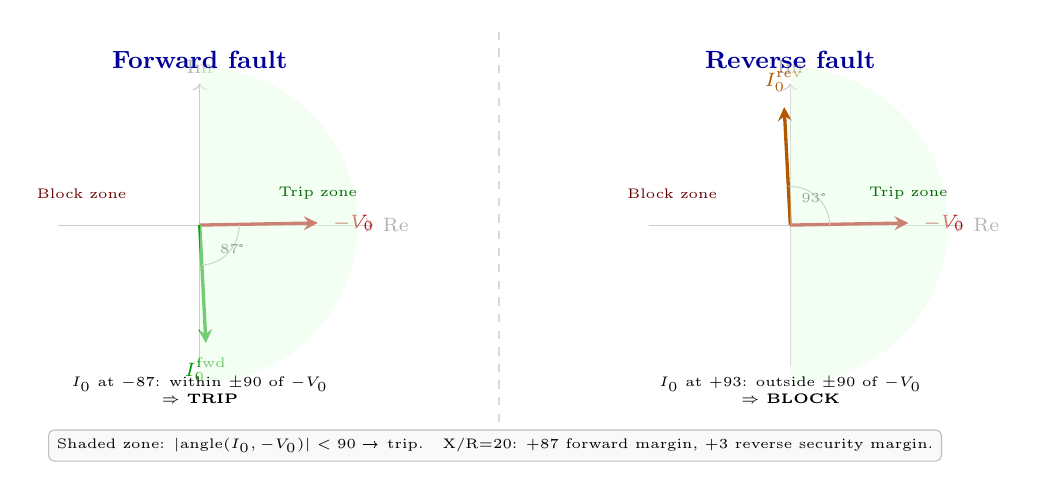
\begin{tikzpicture}[
  every node/.style = {font=\scriptsize},
  vec/.style        = {->, very thick, >=stealth},
  arc/.style        = {draw, thin, gray!60},
]

%% ── Shared scale: 1 unit = normalized phasor length ──────────────────────
\def\Rx{3.5}     % subplot separation
\def\Vs{1.5}     % vector scale

% ── LEFT SUBPLOT: FORWARD FAULT ─────────────────────────────────────────────
\def\ox{0}  \def\oy{0}

% Axes
\draw[gray!40, ->] (\ox-1.8, \oy) -- (\ox+2.2, \oy) node[right,gray!60]{Re};
\draw[gray!40, ->] (\ox, \oy-1.8) -- (\ox, \oy+1.8) node[above,gray!60]{Im};

% -V0 phasor: angle ≈ 0° (positive real, tiny +Im)
\draw[vec, red!70!black]
  (\ox,\oy) -- (\ox+\Vs*0.9998, \oy+\Vs*0.018);
\node[red!70!black, right=2pt] at (\ox+\Vs*0.9998, \oy+\Vs*0.018) {$-V_0$};

% I0 forward phasor: angle ≈ -87° (mostly -Im, tiny +Re)
\draw[vec, green!60!black]
  (\ox,\oy) -- (\ox+\Vs*0.052, \oy-\Vs*0.999);
\node[green!60!black, below=2pt] at (\ox+\Vs*0.052, \oy-\Vs*0.999) {$I_0^\mathrm{fwd}$};

% Arc showing angle between -V0 and I0: ≈ 87°
\draw[arc] (\ox+0.5,\oy) arc[start angle=1, end angle=-87, radius=0.5];
\node[gray!60!black, font=\tiny] at (\ox+0.42, \oy-0.30) {87°};

% Shading: operating zone (±90° of -V0)
\fill[green!10, opacity=0.5]
  (\ox,\oy) -- (\ox, \oy-2.0) arc[start angle=-90, end angle=90, radius=2.0] -- cycle;
\node[green!40!black, font=\tiny] at (\ox+1.5, \oy+0.4) {Trip zone};
\node[red!40!black, font=\tiny] at (\ox-1.5, \oy+0.4) {Block zone};

% Label
\node[font=\small, blue!60!black] at (\ox, \oy+2.1) {\textbf{Forward fault}};
\node[font=\tiny, align=center] at (\ox, \oy-2.1)
  {$I_0$ at $-87°$: within $\pm90°$ of $-V_0$\\$\Rightarrow$ \textbf{TRIP}};

% ── RIGHT SUBPLOT: REVERSE FAULT ────────────────────────────────────────────
\def\ox{7.5}

% Axes
\draw[gray!40, ->] (\ox-1.8, \oy) -- (\ox+2.2, \oy) node[right,gray!60]{Re};
\draw[gray!40, ->] (\ox, \oy-1.8) -- (\ox, \oy+1.8) node[above,gray!60]{Im};

% -V0 phasor: same as forward (bus voltage polarity unchanged)
\draw[vec, red!70!black]
  (\ox,\oy) -- (\ox+\Vs*0.9998, \oy+\Vs*0.018);
\node[red!70!black, right=2pt] at (\ox+\Vs*0.9998, \oy+\Vs*0.018) {$-V_0$};

% I0 reverse phasor: angle ≈ +93° (direction reversed at CT)
\draw[vec, orange!70!black]
  (\ox,\oy) -- (\ox-\Vs*0.052, \oy+\Vs*0.999);
\node[orange!70!black, above=2pt] at (\ox-\Vs*0.052, \oy+\Vs*0.999) {$I_0^\mathrm{rev}$};

% Arc: angle ≈ 93°
\draw[arc] (\ox+0.5,\oy) arc[start angle=1, end angle=93, radius=0.5];
\node[gray!60!black, font=\tiny] at (\ox+0.30, \oy+0.35) {93°};

% Shading: operating zone
\fill[green!10, opacity=0.5]
  (\ox,\oy) -- (\ox, \oy-2.0) arc[start angle=-90, end angle=90, radius=2.0] -- cycle;
\node[green!40!black, font=\tiny] at (\ox+1.5, \oy+0.4) {Trip zone};
\node[red!40!black, font=\tiny] at (\ox-1.5, \oy+0.4) {Block zone};

% Label
\node[font=\small, blue!60!black] at (\ox, \oy+2.1) {\textbf{Reverse fault}};
\node[font=\tiny, align=center] at (\ox, \oy-2.1)
  {$I_0$ at $+93°$: outside $\pm90°$ of $-V_0$\\$\Rightarrow$ \textbf{BLOCK}};

%% ── Divider ──────────────────────────────────────────────────────────────
\draw[gray!30, dashed] (3.8, -2.5) -- (3.8, 2.5);

%% ── Caption note ─────────────────────────────────────────────────────────
\node[draw=gray!50, fill=gray!5, rounded corners=2pt,
      font=\tiny, inner sep=3pt, align=center]
  at (3.75, -2.8)
  {Shaded zone: $|$angle$(I_0, -V_0)| < 90°$ → trip.\quad
   X/R=20: $+87°$ forward margin, $+3°$ reverse security margin.};

\end{tikzpicture}

\end{figure}

% =============================================================================
\section{Coverage Map}
\label{sec:coverage}
% =============================================================================

\begin{figure}[h!]
\centering
\caption{%
  67N\,+\,67Q coverage on the $({\alpha}, k_\mathrm{ibr})$ plane.
  Both elements cover the \emph{entire} plane for $k_\mathrm{ibr} \geq 0.04$\,pu
  (all shown).  The distance relay 21G only operates in the upper-right portion
  (Zone~3, $\alpha \lesssim 0.35$ only, from TR-31).  TR-29 Region~A (red zone,
  below the solid red line) is now covered by 67N/67Q even though 21 is blocked.}
\label{fig:coverage}
% fig_67_coverage.tex
% TR-32: Coverage map on (alpha, k_ibr) plane for 67N+67Q combined scheme
%
% Same axes as TR-29 coverage map: alpha [0,1] x k_ibr [0.06, 0.20]
% Coordinate scaling: x = alpha*10, y = (k_ibr-0.06)/0.14*7
%
% 67N coverage: ALL regions (I0 from network, indep. of k_ibr)
%   colour: green!35 everywhere
%
% 67Q coverage: k_ibr >= I_min_67 = 0.04 pu
%   Since k_ibr range shown is [0.06, 0.20], ALL shown region has k_ibr >= 0.04
%   colour: green!55 (darker, on top of 67N)
%
% Key boundaries (from TR-29):
%   k_ibr = 0.10: 21 I_min threshold (horizontal, red solid)
%   alpha = 0.80: Zone 1 boundary (dash-dot grey)
%
% New boundary for 67Q (not shown in TR-29):
%   k_ibr = 0.04 (67Q lower limit) — below the displayed range

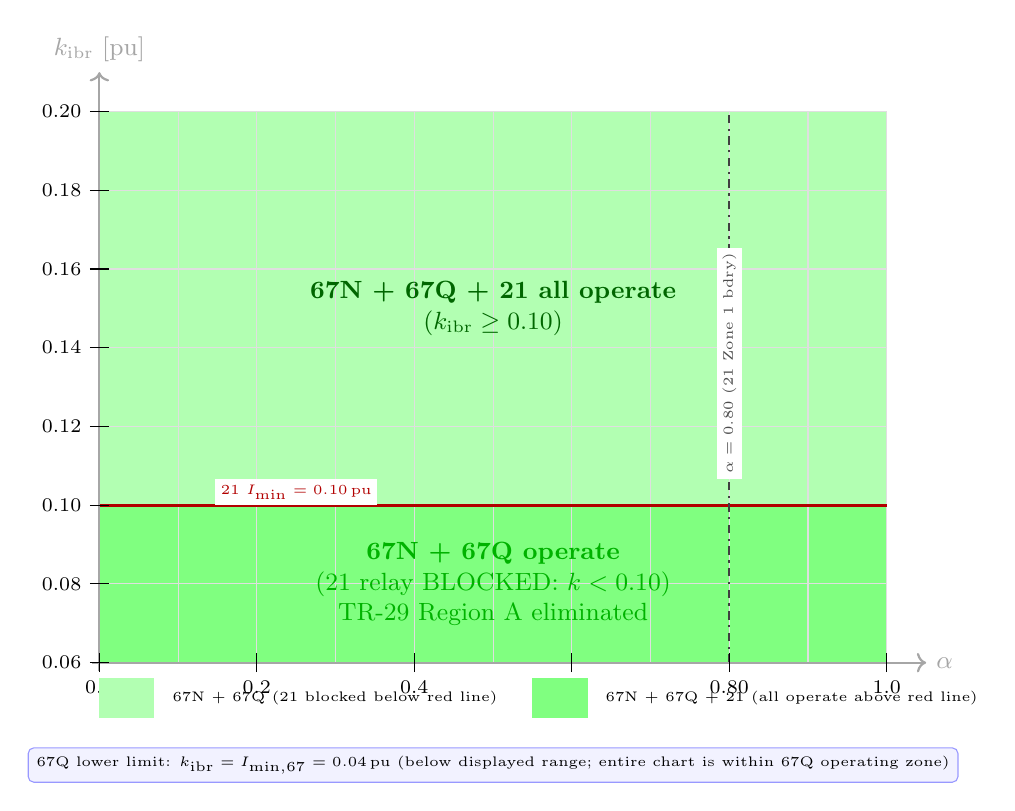
\begin{tikzpicture}[
  every node/.style = {font=\scriptsize},
]

% ── Fill: both 67N and 67Q operate everywhere in the displayed range ──────
\fill[green!30] (0,0) rectangle (10,7);

% ── Highlight: zone where 21 is blocked but 67N/67Q operates ─────────────
% k_ibr < 0.10 → y < (0.10-0.06)/0.14*7 = 2.0
\fill[green!50] (0,0) rectangle (10, 2.0);

% ── Grid ──────────────────────────────────────────────────────────────────
\draw[gray!25, step=1.0] (0,0) grid (10,7);

% ── Boundary lines ────────────────────────────────────────────────────────
% k_ibr = 0.10 (21 I_min threshold)
\draw[red!70!black, very thick] (0, 2.0) -- (10, 2.0);
% alpha = 0.80 (Zone 1 boundary)
\draw[gray!50!black, thick, dash dot] (8.0, 0) -- (8.0, 7.0);

% ── Axes ──────────────────────────────────────────────────────────────────
\draw[->, thick, gray!70] (-0.1, 0) -- (10.5, 0)
  node[right, font=\small] {$\alpha$};
\draw[->, thick, gray!70] (0, -0.1) -- (0, 7.5)
  node[above, font=\small] {$k_\mathrm{ibr}$ [pu]};

\foreach \a/\x in {0.0/0, 0.2/2, 0.4/4, 0.6/6, 0.80/8, 1.0/10} {
  \draw (\x, -0.12) -- (\x, 0.12);
  \node[below=3pt] at (\x, 0) {\a};
}
\foreach \k/\y in {0.06/0, 0.08/1, 0.10/2, 0.12/3, 0.14/4, 0.16/5, 0.18/6, 0.20/7} {
  \draw (-0.12, \y) -- (0.12, \y);
  \node[left=3pt] at (0, \y) {\k};
}

% ── Region labels ─────────────────────────────────────────────────────────
% Lower region (21 blocked, but 67N+67Q OK)
\node[green!70!black, font=\small, align=center] at (5.0, 1.0)
  {\textbf{67N + 67Q operate}\\(21 relay BLOCKED: $k<0.10$)\\TR-29 Region~A eliminated};

% Upper region (all elements operate)
\node[green!40!black, font=\small, align=center] at (5.0, 4.5)
  {\textbf{67N + 67Q + 21 all operate}\\($k_\mathrm{ibr} \geq 0.10$)};

% ── Boundary annotations ──────────────────────────────────────────────────
\node[red!70!black, fill=white, inner sep=2pt, font=\tiny]
  at (2.5, 2.0) [above] {21 $I_\mathrm{min}=0.10$\,pu};

\node[gray!60!black, fill=white, inner sep=2pt, font=\tiny, rotate=90]
  at (8.0, 3.8) {$\alpha=0.80$ (21 Zone~1 bdry)};

% ── 67Q lower limit note (below the chart) ────────────────────────────────
\node[font=\tiny, align=center, draw=blue!40, fill=blue!5,
      rounded corners=2pt, inner sep=3pt]
  at (5.0, -1.3)
  {67Q lower limit: $k_\mathrm{ibr} = I_\mathrm{min,67} = 0.04$\,pu
   (below displayed range; entire chart is within 67Q operating zone)};

% ── Legend ────────────────────────────────────────────────────────────────
\fill[green!30] (0.0, -0.7) rectangle (0.7, -0.2);
\node[right=3pt, font=\tiny] at (0.7, -0.45)
  {67N + 67Q (21 blocked below red line)};

\fill[green!50] (5.5, -0.7) rectangle (6.2, -0.2);
\node[right=3pt, font=\tiny] at (6.2, -0.45)
  {67N + 67Q + 21 (all operate above red line)};

\end{tikzpicture}

\end{figure}

% =============================================================================
\section{Combined Earth-Fault Protection Scheme}
\label{sec:scheme}
% =============================================================================

Combining TR-27 (87L), TR-30 (cross-pol Mho), TR-31 (21G limitations), and
TR-32 (67N/67Q), the recommended IBR earth-fault protection hierarchy is:

\begin{enumerate}
  \item \textbf{Primary instantaneous ($\approx 20$--$30$\,ms):}
        87L chain (elements 87LN0, TDCS) \emph{and} 67N \emph{and} 67Q.
        All three operate in parallel; each is a separate trip path.
        This provides triple redundancy for all $k_\mathrm{ibr} \geq 0.04$\,pu
        and all fault locations $\alpha \in [0,\,1]$.
  \item \textbf{Backup instantaneous Zone~1 ($20$\,ms):}
        Cross-polarised 21 Zone~1 (memory-pol, $\alpha \leq 0.80$,
        $k_\mathrm{ibr} \geq 0.10$\,pu, TR-30).
  \item \textbf{Backup timed Zone~3 ($600$\,ms):}
        Cross-pol 21 Zone~3 via permanent healthy-phase cross-pol
        ($\alpha \lesssim 0.35$ only, as limited by TR-31).
\end{enumerate}

\paragraph{67N/67Q operation time.}
Typical IED implementation: 67N/67Q evaluate the criterion on each cycle
(20\,ms at 50\,Hz) with a 1.5-cycle confirmation window → trip at $\approx 30$\,ms.
This is consistent with the 87L trip time and provides independent redundancy.

% =============================================================================
\section{Conclusions}
\label{sec:conclusions}
% =============================================================================

\begin{enumerate}
  \item The \textbf{active-power directional criterion}
        $\mathrm{Re}[-V_\mathrm{seq}\,I_\mathrm{seq}^*] > 0$ provides reliable
        forward/reverse discrimination for both 67N and 67Q, with margin
        $\Delta = 2\,R_\mathrm{source}\,|I_\mathrm{seq}|^2$.
  \item \textbf{67N operates on $I_0$} (network-sourced, independent of
        $k_\mathrm{ibr}$).  On a purely IBR-fed line, $I_0$ only flows for forward
        faults, so 67N has inherent forward selectivity without needing a
        directional criterion.
  \item \textbf{67Q operates on $I_2 = k_\mathrm{ibr}$} and requires the
        directional criterion.  It operates for all $k_\mathrm{ibr} \geq 0.04$\,pu
        --- extending coverage 60\% below the distance relay $I_\mathrm{min}$.
  \item \textbf{TR-29 Region~A is eliminated} for earth faults: 67N/67Q cover the
        full $({\alpha},\,k_\mathrm{ibr})$ plane without any blocked zone.
  \item \textbf{Combined scheme} 87L\,$+$\,67N\,$+$\,67Q provides triple
        redundancy for all IBR SLG faults at $\approx 20$--$30$\,ms, fully
        independent of the 21G $k_0$ measurement limitation (TR-31).
\end{enumerate}

\bibliographystyle{IEEEtran}
\bibliography{references32}

\end{document}
